\documentclass{beamer}

\usepackage{amsfonts}
\usepackage{amsmath}
\usepackage{amssymb}
\usepackage{amsthm}
\usepackage{caption}
\usepackage{hyperref}
\usepackage[indent=0pt]{parskip}

\usepackage{natbib}
\bibliographystyle{abbrvnat}
\setcitestyle{authoryear,open={(},close={)}} %Citation-related commands
\usepackage{tikz}
\usetikzlibrary{graphs}

\usepackage[dvipsnames]{xcolor}
\definecolor{tmublue}{RGB}{0, 76, 155}
\definecolor{tmuyellow}{RGB}{255, 220, 0}
\definecolor{darkblue}{RGB}{0, 45, 114}
\definecolor{medblue}{RGB}{0, 119, 200}

%Information to be included in the title page:
\title{\color{darkblue}\LARGE Improving Community Detection via Community Association Strength Sores}
\subtitle{\color{darkblue} \vspace{2em} WAW 2025}
\author{\color{darkblue} Jordan Barrett$^*$, \textbf{Ryan DeWolfe}$^*$, Bogumił Kamiński$^\dagger$,\\ Paweł Prałat$^*$, Aaron Smith$^\ddagger$, and François Théberge$^\mathparagraph$.}
\institute{\color{darkblue}
    $^*$Toronto Metropolitan University\\
    $^\dagger$SGH Warsaw School of Economics\\
    $^\ddagger$University of Ottawa\\
    $^\mathparagraph$Tutte Institute for Mathematics and Computing
}
\date{\color{darkblue}July 2025}

\begin{document}
\color{darkblue} % Global default color
\setbeamercolor*{enumerate item}{fg=darkblue}
\setbeamercolor*{itemize item}{fg=darkblue}
\setbeamercolor*{caption name}{fg=darkblue}
\setbeamercolor*{caption}{fg=darkblue}
\renewcommand{\subtitle}[1]{
    {
    \setbeamercolor{background canvas}{bg=darkblue}
    \begin{frame}
        \vspace*{\stretch{1}}
        \centering
        \textcolor{white}{\bf\Huge#1}
        \vspace{\stretch{1}}
    \end{frame}
    }
}
\newcommand{\slidetitle}[1]{
    \textcolor{tmublue}{\LARGE#1}
}
\addtobeamertemplate{navigation symbols}{}{%
    \usebeamerfont{Large}%
    \usebeamercolor[fg]{footline}%
    \hspace{1em}%
    \insertframenumber/\inserttotalframenumber
}

\frame{\titlepage}

\begin{frame}{\slidetitle{Motivation}}
    \begin{figure}
    \centering
    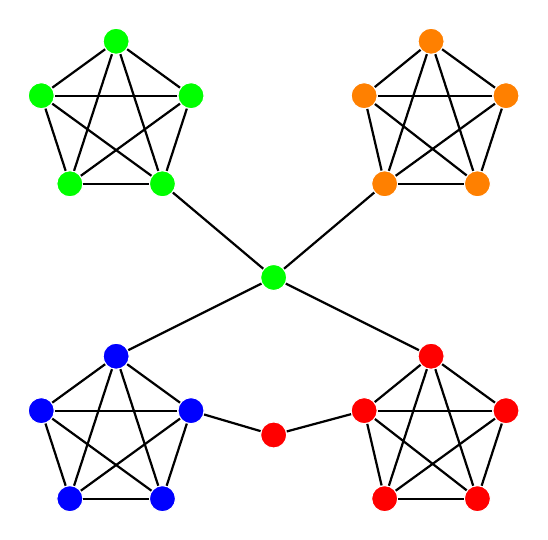
\begin{tikzpicture}
        \begin{scope}[
            every node/.style={shape=circle,draw=white}
        ]
            \node[fill=blue] (A1) at (0, 1) {};
            \node[fill=blue] (B1) at (0.951, 0.309) {};
            \node[fill=blue] (C1) at (0.588, -0.809) {};
            \node[fill=blue] (D1) at (-0.588, -0.809) {};
            \node[fill=blue] (E1) at (-0.951, 0.309) {};

            \node[fill=red] (A2) at (4, 1) {};
            \node[fill=red] (B2) at (4.951, 0.309) {};
            \node[fill=red] (C2) at (4.588, -0.809) {};
            \node[fill=red] (D2) at (3.41, -0.809) {};
            \node[fill=red] (E2) at (3.15, 0.309) {};

            \node[fill=green] (A3) at (0, 5) {};
            \node[fill=green] (B3) at (0.951, 4.309) {};
            \node[fill=green] (C3) at (0.588, 3.19) {};
            \node[fill=green] (D3) at (-0.588, 3.19) {};
            \node[fill=green] (E3) at (-0.951, 4.309) {};

            \node[fill=orange] (A4) at (4, 5) {};
            \node[fill=orange] (B4) at (4.951, 4.309) {};
            \node[fill=orange] (C4) at (4.588, 3.19) {};
            \node[fill=orange] (D4) at (3.41, 3.19) {};
            \node[fill=orange] (E4) at (3.15, 4.309) {};

            \node[fill=green] (O1) at (2,2) {};
            \node[fill=red] (O2) at (2,0) {};
        \end{scope}
        \begin{scope}[
            every node/.style={fill=white,circle},
            every edge/.style={draw=black,thick}
        ]
            \path [-] (A1) edge (B1);
            \path [-] (A1) edge (C1);
            \path [-] (A1) edge (D1);
            \path [-] (A1) edge (E1);
            \path [-] (B1) edge (C1);
            \path [-] (B1) edge (D1);
            \path [-] (B1) edge (E1);
            \path [-] (C1) edge (D1);
            \path [-] (C1) edge (E1);
            \path [-] (D1) edge (E1);

            \path [-] (A2) edge (B2);
            \path [-] (A2) edge (C2);
            \path [-] (A2) edge (D2);
            \path [-] (A2) edge (E2);
            \path [-] (B2) edge (C2);
            \path [-] (B2) edge (D2);
            \path [-] (B2) edge (E2);
            \path [-] (C2) edge (D2);
            \path [-] (C2) edge (E2);
            \path [-] (D2) edge (E2);

            \path [-] (A3) edge (B3);
            \path [-] (A3) edge (C3);
            \path [-] (A3) edge (D3);
            \path [-] (A3) edge (E3);
            \path [-] (B3) edge (C3);
            \path [-] (B3) edge (D3);
            \path [-] (B3) edge (E3);
            \path [-] (C3) edge (D3);
            \path [-] (C3) edge (E3);
            \path [-] (D3) edge (E3);

            \path [-] (A4) edge (B4);
            \path [-] (A4) edge (C4);
            \path [-] (A4) edge (D4);
            \path [-] (A4) edge (E4);
            \path [-] (B4) edge (C4);
            \path [-] (B4) edge (D4);
            \path [-] (B4) edge (E4);
            \path [-] (C4) edge (D4);
            \path [-] (C4) edge (E4);
            \path [-] (D4) edge (E4);

            \path [-] (O1) edge (A1);
            \path [-] (O1) edge (A2);
            \path [-] (O1) edge (C3);
            \path [-] (O1) edge (D4);

            \path [-] (O2) edge (B1);
            \path [-] (O2) edge (E2);
        \end{scope}
    \end{tikzpicture}
    \vspace{1em}
    \caption{An example of a partition.}
    \end{figure}
\end{frame}

\begin{frame}{\slidetitle{Agenda}}
    \begin{enumerate}
        \color{darkblue}
        \item CAS Scores
        \item Properties of CAS Scores
        \item Applications:\\
            \vspace{0.5em}
            \begin{enumerate}
                \color{darkblue}
                \item Improving Partitons
                \item Detecting Outliers
                \item Overlapping Communities
            \end{enumerate}
    \end{enumerate}
\end{frame}

\subtitle{The Scores}

\begin{frame}{\slidetitle{Proposed Scores}}
    \large{Internal Edge Fraction:}
    $$\mathrm{IEF}(v, C) := \frac{\deg_C(v)}{\deg(v)}.$$
    \begin{minipage}{0.6\linewidth}
    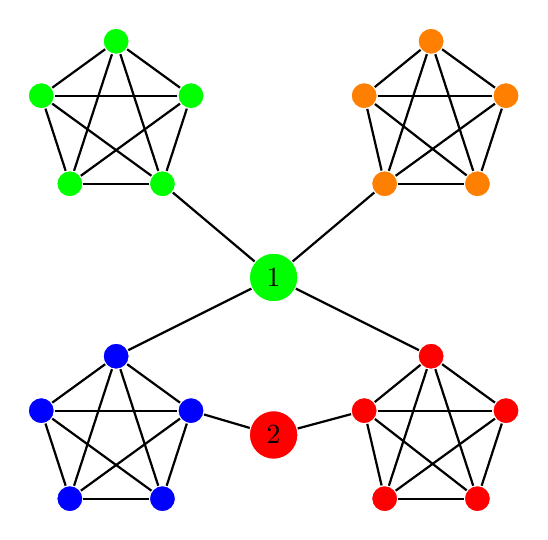
\begin{tikzpicture}
        \begin{scope}[
            every node/.style={shape=circle,draw=white}
        ]
            \node[fill=blue] (A1) at (0, 1) {};
            \node[fill=blue] (B1) at (0.951, 0.309) {};
            \node[fill=blue] (C1) at (0.588, -0.809) {};
            \node[fill=blue] (D1) at (-0.588, -0.809) {};
            \node[fill=blue] (E1) at (-0.951, 0.309) {};

            \node[fill=red] (A2) at (4, 1) {};
            \node[fill=red] (B2) at (4.951, 0.309) {};
            \node[fill=red] (C2) at (4.588, -0.809) {};
            \node[fill=red] (D2) at (3.41, -0.809) {};
            \node[fill=red] (E2) at (3.15, 0.309) {};

            \node[fill=green] (A3) at (0, 5) {};
            \node[fill=green] (B3) at (0.951, 4.309) {};
            \node[fill=green] (C3) at (0.588, 3.19) {};
            \node[fill=green] (D3) at (-0.588, 3.19) {};
            \node[fill=green] (E3) at (-0.951, 4.309) {};

            \node[fill=orange] (A4) at (4, 5) {};
            \node[fill=orange] (B4) at (4.951, 4.309) {};
            \node[fill=orange] (C4) at (4.588, 3.19) {};
            \node[fill=orange] (D4) at (3.41, 3.19) {};
            \node[fill=orange] (E4) at (3.15, 4.309) {};

            \node[fill=green] (O1) at (2,2) {1};
            \node[fill=red] (O2) at (2,0) {2};
        \end{scope}
        \begin{scope}[
            every node/.style={fill=white,circle},
            every edge/.style={draw=black,thick}
        ]
            \path [-] (A1) edge (B1);
            \path [-] (A1) edge (C1);
            \path [-] (A1) edge (D1);
            \path [-] (A1) edge (E1);
            \path [-] (B1) edge (C1);
            \path [-] (B1) edge (D1);
            \path [-] (B1) edge (E1);
            \path [-] (C1) edge (D1);
            \path [-] (C1) edge (E1);
            \path [-] (D1) edge (E1);

            \path [-] (A2) edge (B2);
            \path [-] (A2) edge (C2);
            \path [-] (A2) edge (D2);
            \path [-] (A2) edge (E2);
            \path [-] (B2) edge (C2);
            \path [-] (B2) edge (D2);
            \path [-] (B2) edge (E2);
            \path [-] (C2) edge (D2);
            \path [-] (C2) edge (E2);
            \path [-] (D2) edge (E2);

            \path [-] (A3) edge (B3);
            \path [-] (A3) edge (C3);
            \path [-] (A3) edge (D3);
            \path [-] (A3) edge (E3);
            \path [-] (B3) edge (C3);
            \path [-] (B3) edge (D3);
            \path [-] (B3) edge (E3);
            \path [-] (C3) edge (D3);
            \path [-] (C3) edge (E3);
            \path [-] (D3) edge (E3);

            \path [-] (A4) edge (B4);
            \path [-] (A4) edge (C4);
            \path [-] (A4) edge (D4);
            \path [-] (A4) edge (E4);
            \path [-] (B4) edge (C4);
            \path [-] (B4) edge (D4);
            \path [-] (B4) edge (E4);
            \path [-] (C4) edge (D4);
            \path [-] (C4) edge (E4);
            \path [-] (D4) edge (E4);

            \path [-] (O1) edge (A1);
            \path [-] (O1) edge (A2);
            \path [-] (O1) edge (C3);
            \path [-] (O1) edge (D4);

            \path [-] (O2) edge (B1);
            \path [-] (O2) edge (E2);
        \end{scope}
    \end{tikzpicture}
    \end{minipage}
    \begin{minipage}{0.35\linewidth}
        \begin{align*}
            &IEF(1, ``GREEN") = \frac{1}{4}\\
            &IEF(2, ``RED")  = \frac{1}{2}\\
            &IEF(2, ``BLUE") = \frac{1}{2}\\
        \end{align*}
    \end{minipage}
\end{frame}

\begin{frame}{\slidetitle{Proposed Scores}}
    \large{Normalized Internal Edge Fraction:}
    $$\mathrm{NIEF}(v, C) := \max\left\{ \mathrm{IEF}(v, C) - \frac{vol(C)}{vol{V}} , 0 \right\}.$$
    \begin{minipage}{0.57\linewidth}
    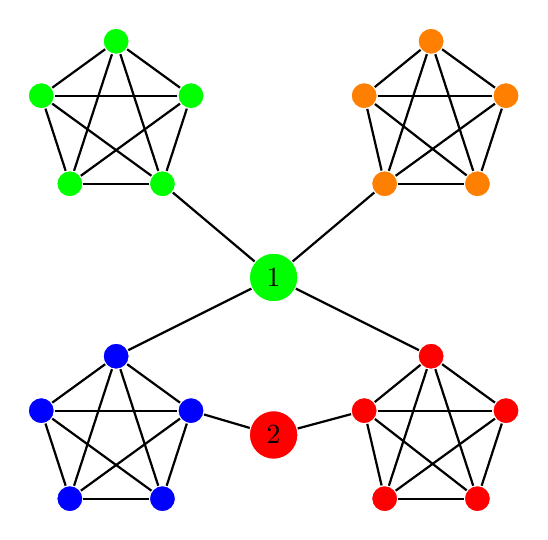
\begin{tikzpicture}
        \begin{scope}[
            every node/.style={shape=circle,draw=white}
        ]
            \node[fill=blue] (A1) at (0, 1) {};
            \node[fill=blue] (B1) at (0.951, 0.309) {};
            \node[fill=blue] (C1) at (0.588, -0.809) {};
            \node[fill=blue] (D1) at (-0.588, -0.809) {};
            \node[fill=blue] (E1) at (-0.951, 0.309) {};

            \node[fill=red] (A2) at (4, 1) {};
            \node[fill=red] (B2) at (4.951, 0.309) {};
            \node[fill=red] (C2) at (4.588, -0.809) {};
            \node[fill=red] (D2) at (3.41, -0.809) {};
            \node[fill=red] (E2) at (3.15, 0.309) {};

            \node[fill=green] (A3) at (0, 5) {};
            \node[fill=green] (B3) at (0.951, 4.309) {};
            \node[fill=green] (C3) at (0.588, 3.19) {};
            \node[fill=green] (D3) at (-0.588, 3.19) {};
            \node[fill=green] (E3) at (-0.951, 4.309) {};

            \node[fill=orange] (A4) at (4, 5) {};
            \node[fill=orange] (B4) at (4.951, 4.309) {};
            \node[fill=orange] (C4) at (4.588, 3.19) {};
            \node[fill=orange] (D4) at (3.41, 3.19) {};
            \node[fill=orange] (E4) at (3.15, 4.309) {};

            \node[fill=green] (O1) at (2,2) {1};
            \node[fill=red] (O2) at (2,0) {2};
        \end{scope}
        \begin{scope}[
            every node/.style={fill=white,circle},
            every edge/.style={draw=black,thick}
        ]
            \path [-] (A1) edge (B1);
            \path [-] (A1) edge (C1);
            \path [-] (A1) edge (D1);
            \path [-] (A1) edge (E1);
            \path [-] (B1) edge (C1);
            \path [-] (B1) edge (D1);
            \path [-] (B1) edge (E1);
            \path [-] (C1) edge (D1);
            \path [-] (C1) edge (E1);
            \path [-] (D1) edge (E1);

            \path [-] (A2) edge (B2);
            \path [-] (A2) edge (C2);
            \path [-] (A2) edge (D2);
            \path [-] (A2) edge (E2);
            \path [-] (B2) edge (C2);
            \path [-] (B2) edge (D2);
            \path [-] (B2) edge (E2);
            \path [-] (C2) edge (D2);
            \path [-] (C2) edge (E2);
            \path [-] (D2) edge (E2);

            \path [-] (A3) edge (B3);
            \path [-] (A3) edge (C3);
            \path [-] (A3) edge (D3);
            \path [-] (A3) edge (E3);
            \path [-] (B3) edge (C3);
            \path [-] (B3) edge (D3);
            \path [-] (B3) edge (E3);
            \path [-] (C3) edge (D3);
            \path [-] (C3) edge (E3);
            \path [-] (D3) edge (E3);

            \path [-] (A4) edge (B4);
            \path [-] (A4) edge (C4);
            \path [-] (A4) edge (D4);
            \path [-] (A4) edge (E4);
            \path [-] (B4) edge (C4);
            \path [-] (B4) edge (D4);
            \path [-] (B4) edge (E4);
            \path [-] (C4) edge (D4);
            \path [-] (C4) edge (E4);
            \path [-] (D4) edge (E4);

            \path [-] (O1) edge (A1);
            \path [-] (O1) edge (A2);
            \path [-] (O1) edge (C3);
            \path [-] (O1) edge (D4);

            \path [-] (O2) edge (B1);
            \path [-] (O2) edge (E2);
        \end{scope}
    \end{tikzpicture}
    \end{minipage}
    \begin{minipage}{0.4\linewidth}
        \begin{align*}
            &NIEF(1, ``GREEN") = 0\\
            &NIEF(2, ``RED")  = 0.24\\
            &NIEF(2, ``BLUE") = 0.26\\
        \end{align*}
    \end{minipage}
\end{frame}

\begin{frame}{\slidetitle{Proposed scores}}
    The motivation for P.
    \begin{itemize}
        \color{darkblue}
        \item The probability of an edge from $v$ into $C$ in a resampling of $G$ is $w(C)$.
        \item There are $deg(v)$ edges from $v$.
        \item $1 - P(v, C)$ is the probability that at least $deg_C(v)$ edges are into $C$ after a resampling.
        \item Let $F(\cdot; n, p)$ be the CDF of the binomial distribution with parameters $n$ and $p$.
        \item $P(v,c) = F\left(\deg_C(v) - 1; \deg(v), \frac{vol(C)}{vol(V)} \right)$
    \end{itemize}
\end{frame}

\begin{frame}{\slidetitle{Proposed Scores}}
    \large{P:}
    $$\mathrm{P}(v, C) := F\left(\deg_C(v) - 1; \deg(v), \frac{vol(C)}{vol(V)} \right).$$
    \begin{minipage}{0.6\linewidth}
    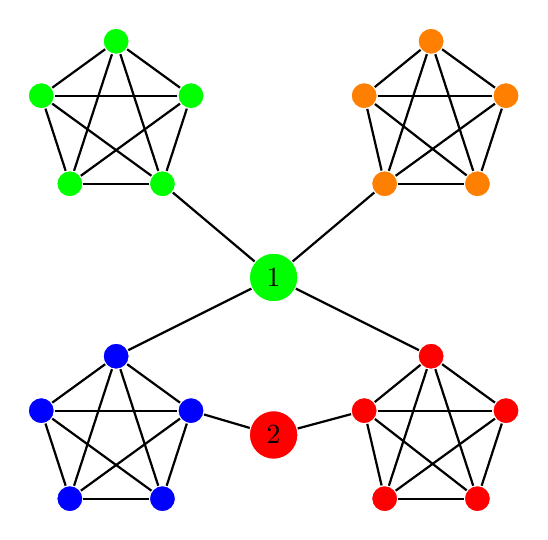
\begin{tikzpicture}
        \begin{scope}[
            every node/.style={shape=circle,draw=white}
        ]
            \node[fill=blue] (A1) at (0, 1) {};
            \node[fill=blue] (B1) at (0.951, 0.309) {};
            \node[fill=blue] (C1) at (0.588, -0.809) {};
            \node[fill=blue] (D1) at (-0.588, -0.809) {};
            \node[fill=blue] (E1) at (-0.951, 0.309) {};

            \node[fill=red] (A2) at (4, 1) {};
            \node[fill=red] (B2) at (4.951, 0.309) {};
            \node[fill=red] (C2) at (4.588, -0.809) {};
            \node[fill=red] (D2) at (3.41, -0.809) {};
            \node[fill=red] (E2) at (3.15, 0.309) {};

            \node[fill=green] (A3) at (0, 5) {};
            \node[fill=green] (B3) at (0.951, 4.309) {};
            \node[fill=green] (C3) at (0.588, 3.19) {};
            \node[fill=green] (D3) at (-0.588, 3.19) {};
            \node[fill=green] (E3) at (-0.951, 4.309) {};

            \node[fill=orange] (A4) at (4, 5) {};
            \node[fill=orange] (B4) at (4.951, 4.309) {};
            \node[fill=orange] (C4) at (4.588, 3.19) {};
            \node[fill=orange] (D4) at (3.41, 3.19) {};
            \node[fill=orange] (E4) at (3.15, 4.309) {};

            \node[fill=green] (O1) at (2,2) {1};
            \node[fill=red] (O2) at (2,0) {2};
        \end{scope}
        \begin{scope}[
            every node/.style={fill=white,circle},
            every edge/.style={draw=black,thick}
        ]
            \path [-] (A1) edge (B1);
            \path [-] (A1) edge (C1);
            \path [-] (A1) edge (D1);
            \path [-] (A1) edge (E1);
            \path [-] (B1) edge (C1);
            \path [-] (B1) edge (D1);
            \path [-] (B1) edge (E1);
            \path [-] (C1) edge (D1);
            \path [-] (C1) edge (E1);
            \path [-] (D1) edge (E1);

            \path [-] (A2) edge (B2);
            \path [-] (A2) edge (C2);
            \path [-] (A2) edge (D2);
            \path [-] (A2) edge (E2);
            \path [-] (B2) edge (C2);
            \path [-] (B2) edge (D2);
            \path [-] (B2) edge (E2);
            \path [-] (C2) edge (D2);
            \path [-] (C2) edge (E2);
            \path [-] (D2) edge (E2);

            \path [-] (A3) edge (B3);
            \path [-] (A3) edge (C3);
            \path [-] (A3) edge (D3);
            \path [-] (A3) edge (E3);
            \path [-] (B3) edge (C3);
            \path [-] (B3) edge (D3);
            \path [-] (B3) edge (E3);
            \path [-] (C3) edge (D3);
            \path [-] (C3) edge (E3);
            \path [-] (D3) edge (E3);

            \path [-] (A4) edge (B4);
            \path [-] (A4) edge (C4);
            \path [-] (A4) edge (D4);
            \path [-] (A4) edge (E4);
            \path [-] (B4) edge (C4);
            \path [-] (B4) edge (D4);
            \path [-] (B4) edge (E4);
            \path [-] (C4) edge (D4);
            \path [-] (C4) edge (E4);
            \path [-] (D4) edge (E4);

            \path [-] (O1) edge (A1);
            \path [-] (O1) edge (A2);
            \path [-] (O1) edge (C3);
            \path [-] (O1) edge (D4);

            \path [-] (O2) edge (B1);
            \path [-] (O2) edge (E2);
        \end{scope}
    \end{tikzpicture}
    \end{minipage}
    \begin{minipage}{0.35\linewidth}
        \begin{align*}
            &P(1, ``GREEN") = 0.28\\
            &P(2, ``RED")  = 0.55\\
            &P(2, ``BLUE") = 0.58\\
        \end{align*}
    \end{minipage}
\end{frame}

\subtitle{Properties}

\begin{frame}{\slidetitle{Properties of CAS}}
    \large
    \begin{enumerate}
        \color{darkblue}
        \item All scores are $0$ if there are no edges into a community.
        \item For a fixed $vol(C)$, all scores are monotone increasing with $deg_C$.
    \end{enumerate}
    \vspace{1em}
    Both of these properties are intuitive.
    A further research direction is finding a larger set of intuitive properties that could narrow the set of acceptable CAS scores.
\end{frame}

\begin{frame}{\slidetitle{Properties of CAS}}
Consider the following graph transformations:
    \begin{enumerate}
        \color{darkblue}
        \item Add a new community this is disjoint to the original graph.
        \item Create a copy of each edge. (Since the CAS scores only depend on $deg_C(v)$ and $vol(C)$, this can be replaced with doubling each of these values by creating new edges.)
    \end{enumerate}
    \vspace{1em}
    \begin{table}
        \centering
        \begin{tabular}{c|c|c|c}
            Transformation & IEF & NIEF & P\\ \hline
            1 & Unchanged & Increases & Increases \\
            2 & Unchanged & Unchanged & ``More Extreme''
        \end{tabular}
    \end{table}
\end{frame}

\subtitle{Applications}

\begin{frame}{\slidetitle{Data}}
    We use $\mathbf{ABCD}$ \citep{abcd}, $\mathbf{ABCD+o}$ \citep{abcdo}, and $\mathbf{ABCD+o^2}$ \citep{abcdoo} synthetic graphs for evaluation.
    \begin{figure}
        \centering
        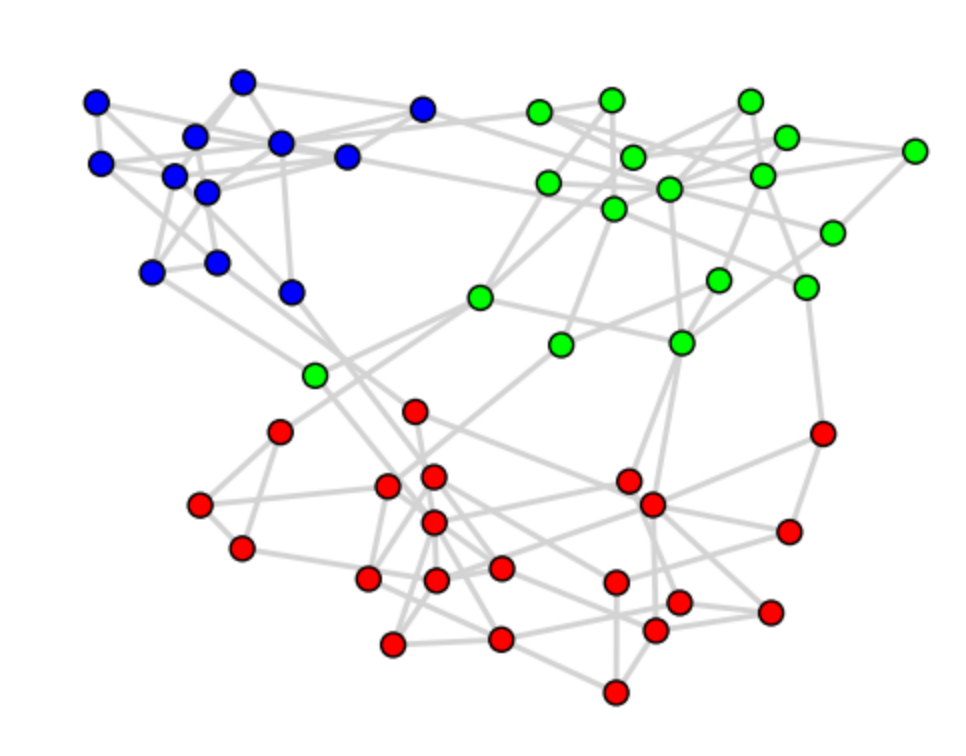
\includegraphics[height=0.6\textheight]{figures/abcd.png}
        \caption{Example ABCD graph with $n=50, \xi=0.2$.}
    \end{figure}
\end{frame}
\begin{frame}{\slidetitle{Data}}
    We also consider the Football graph \citep{football} as an example of real data with known outliers.
    \begin{figure}
        \centering
        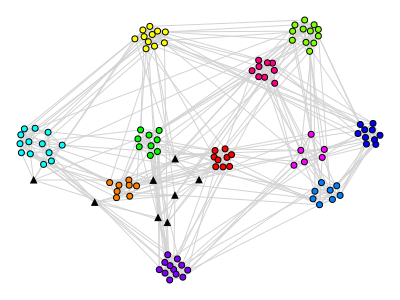
\includegraphics[height=0.6\textheight]{figures/foot1b.png}
        \caption{The football graph colored by conference.}
    \end{figure}
\end{frame}

\subtitle{Improving Partitions}

\begin{frame}{\slidetitle{Improved ECG}}
    The very successful ECG \citep{ecg} community detection algorithm works as follows:
    \begin{enumerate}
        \color{darkblue}
        \item Perform 1-iteration of the Louvain algorithm $k$ times to get $k$ partitions.
        \item Weight each edge $uv$ as the average of the indicator $\chi(u \text{ and } v  \text{ are in the same community})$ from step 1.
        \item Run Louvain or Leiden on this weighted graph.
    \end{enumerate}
\end{frame}
\begin{frame}{\slidetitle{Improved ECG}}
    We rewrite step 2 using CAS scores.
    \begin{enumerate}
        \color{darkblue}
        \item Perform 1-iteration of the Louvain algorithm $k$ times to get $k$ partitions.
        \item Weight each edge $uv$ as the average of $CAS(uv)$ from step 1.
        \item Run Louvain or Leiden on this weighted graph.
    \end{enumerate}
    With the option of any CAS score and two options to symmetrise:
    $$CAS_{or}(uv) = CAS(u, C_v) + CAS(v, C_u) - CAS(u,C_v) \cdot CAS(v,C_u)$$
    $$CAS_{and}(uv) = CAS(u,C_v) \cdot CAS(v,C_u)$$
\end{frame}
\begin{frame}{\slidetitle{Improved ECG}}
    \begin{figure}
        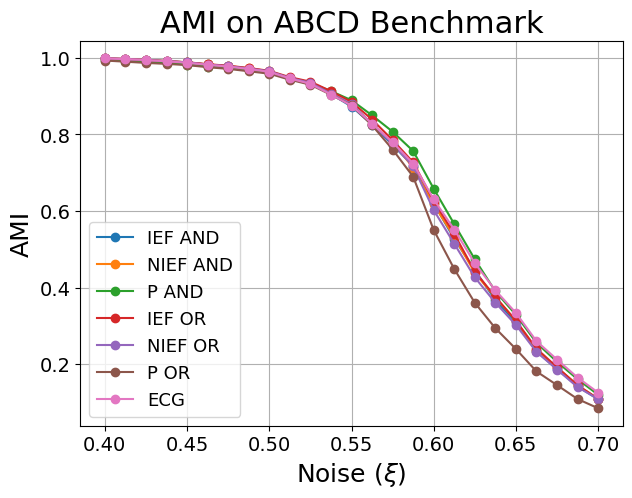
\includegraphics[height=0.8\textheight]{figures/ami-cas-ecg.png}
        \caption{AMI of the proposed CAS-ECG methods.}
    \end{figure}
\end{frame}
\begin{frame}{\slidetitle{Improved ECG}}
    \begin{figure}
        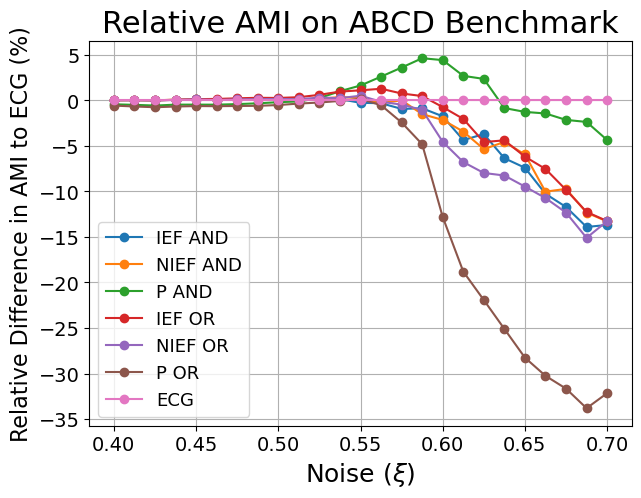
\includegraphics[height=0.8\textheight]{figures/relative-ami-cas-ecg.png}
        \caption{AMI of the proposed CAS-ECG methods compared to ECG.}
    \end{figure}
\end{frame}

\subtitle{Detecting Outliers}

\begin{frame}{\slidetitle{Detecting Outliers}}
    \begin{itemize}
        \color{darkblue}
        \item Suppose some nodes are not strongly associated to any community (outliers).
        \item We test if the maximum CAS to any community can predict if a node is not an outlier.
    \end{itemize}
    $$\lnot outlier(v) = \max_{C\in \mathcal{C}} CAS(v,C)$$
\end{frame}
\begin{frame}{\slidetitle{Detecting Outliers}}
    \begin{figure}
        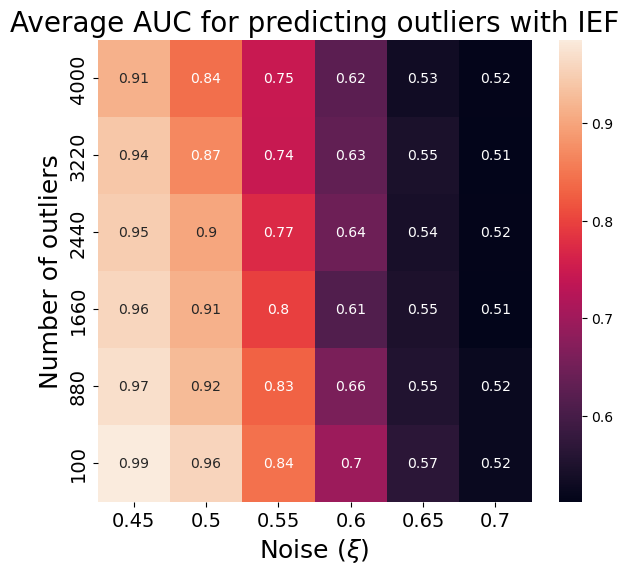
\includegraphics[height=0.75\textheight]{figures/outlier-auc-ief.png}
        \caption{Classifing ABCD+o outliers with CAS.}
    \end{figure}
\end{frame}
\begin{frame}{\slidetitle{Detecting Outliers}}
    \begin{figure}
        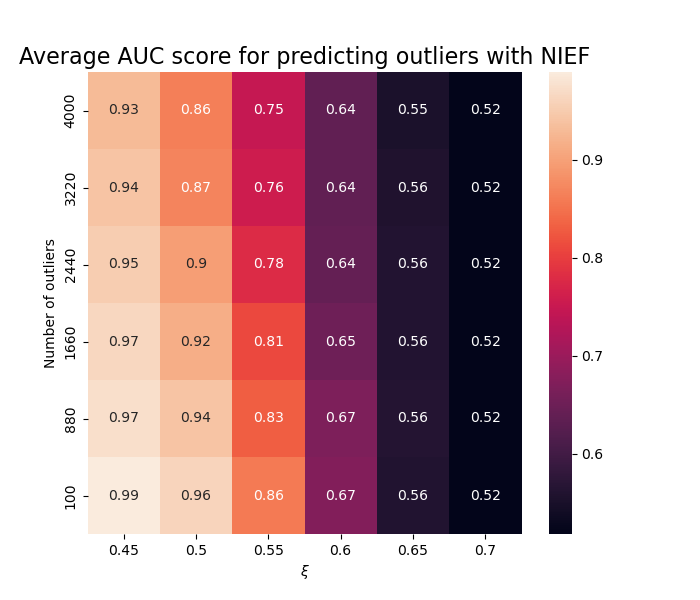
\includegraphics[height=0.9\textheight]{figures/outlier-auc-nief.png}
        \caption{Classifing ABCD+o outliers with CAS.}
    \end{figure}
\end{frame}
\begin{frame}{\slidetitle{Detecting Outliers}}
    \begin{figure}
        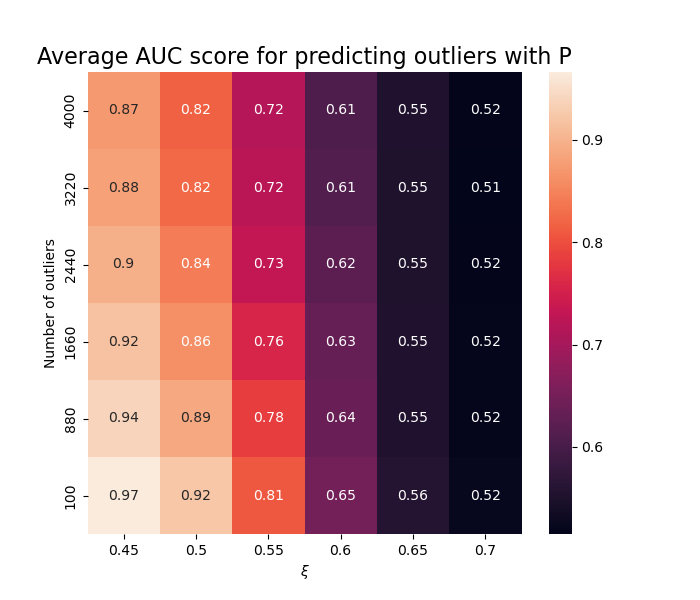
\includegraphics[height=0.9\textheight]{figures/outlier-auc-p.png}
        \caption{Classifing ABCD+o outliers with CAS.}
    \end{figure}
\end{frame}
\begin{frame}{\slidetitle{Detecting Outliers}}
    \begin{figure}
        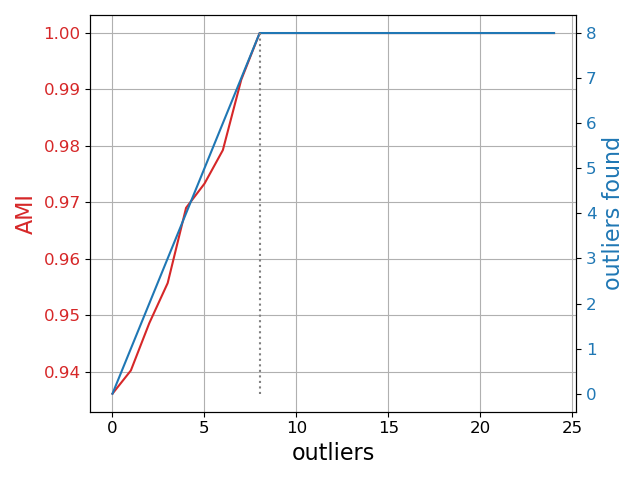
\includegraphics[height=0.8\textheight]{figures/foot2b.png}
        \caption{Classifying Football outliers with $P$.}
    \end{figure}
\end{frame}

\subtitle{Overlapping Communities}

\begin{frame}{\slidetitle{Overlapping Communities}}
    \begin{enumerate}
        \color{darkblue}
        \item We start with some set of (possibly overlapping communities) $\mathcal{C} = \{C_1, C_2, \dots C_k\}$.
        \item Construct a new collection of communities $\mathcal{C}'$ where $C_i' = \{v: CAS(v, C_i \geq \tau)\}$.
    \end{enumerate}
    We use ego-split \citep{egosplit} to find the initial communities, and we find $\tau \in [0.075,0.25]$ improves the communities when compared to the true labels with oNMI \citep{onmi}.
\end{frame}
\begin{frame}{\slidetitle{Overlapping Communities}}
    \begin{figure}
        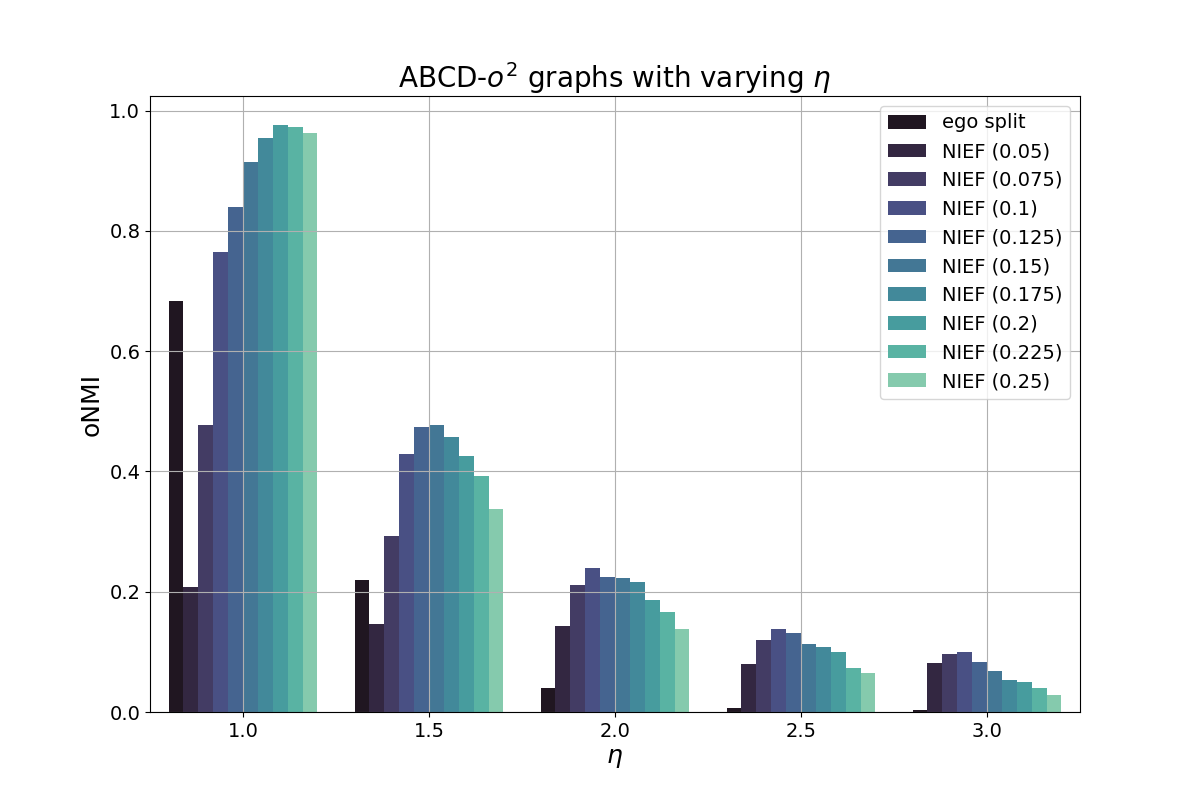
\includegraphics[height=0.7\textheight]{figures/ego_1.png}
        \caption{Using NIEF to post-process Ego-split.}
    \end{figure}
\end{frame}
\begin{frame}{\slidetitle{Overlapping Communities}}
    \begin{figure}
        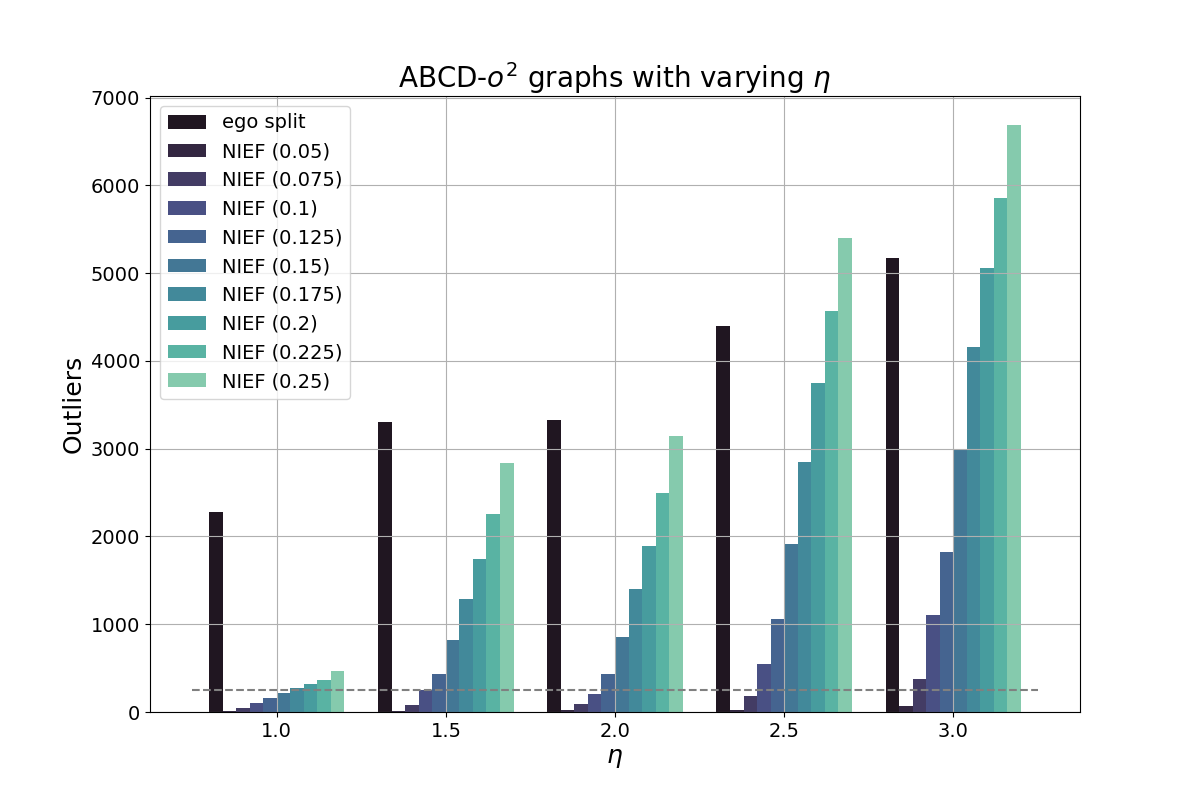
\includegraphics[height=0.7\textheight]{figures/ego_2.png}
        \caption{Using NIEF to post-process Ego-split.}
    \end{figure}
\end{frame}
\begin{frame}{\slidetitle{Overlapping Communities}}
    \begin{figure}
        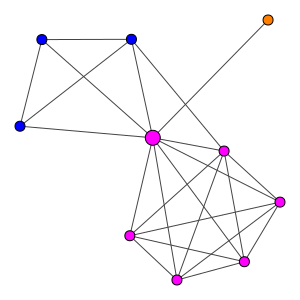
\includegraphics[width=0.49\linewidth]{figures/foot3a.png} \hfill
        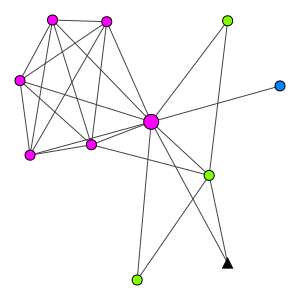
\includegraphics[width=0.49\linewidth]{figures/foot3b.png}
        \caption{Ego-nets of nodes with potential overlap using CAS-ECG and $P$ from the football graph.}
    \end{figure}
\end{frame}

\begin{frame}{\slidetitle{Bonus Application: Layouts}}
    \begin{figure}
        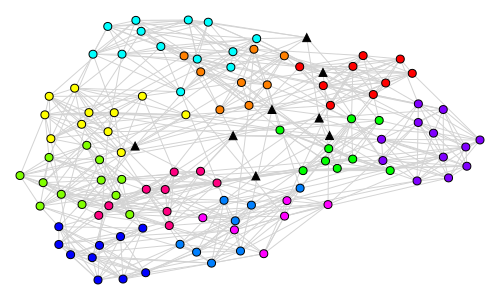
\includegraphics[width=0.49\linewidth]{figures/foot1a.png} \hfill
        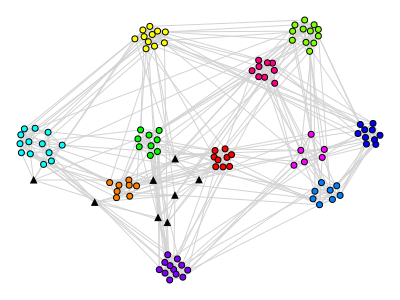
\includegraphics[width=0.49\linewidth]{figures/foot1b.png}
        \vspace{1em}
        \caption{Force-direct layout of the football graph with (right) and without (left) edge weighting using CAS-ECG.}
    \end{figure}
\end{frame}

\begin{frame}{\slidetitle{Summary}}
    \begin{itemize}
        \color{darkblue}
        \item There are several options for community association strength scores.
        \item They are useful for improving a variety of community detection tasks.
        \item Post-processing techniques appear to be a viable approach to outlier detection and overlapping communities.
    \end{itemize}
\end{frame}

\begin{frame}[allowframebreaks]{\slidetitle{References}}
    \bibliography{references}
\end{frame}

\end{document}